\documentclass{article}

\usepackage{amsmath}
\usepackage{booktabs}
\usepackage{float}
\usepackage{tabularx}
\usepackage{soul, color}

\newcolumntype{I}{>{\centering\arraybackslash\hsize=.4\hsize}X}


\usepackage{amsmath,amsthm,amssymb}
\usepackage{mathtext}
\usepackage[T2A]{fontenc}
\usepackage[utf8]{inputenc}
\usepackage[english]{babel}
\usepackage{graphicx}
\usepackage{hyperref}


\title{Semantic search of similar academic papers}
\author{Alexander Demidovskij \and Igor Salnikov}
\date{December 2023}



\begin{document}
\maketitle

\begin{abstract}
    Information retrieval is one of the integral parts of modern natural language processing tasks. arXiv is one of the key resources nowadays for sharing the latest and greatest results in various academic fields, such as computer science. However, the built-in search on the website does not allow for the most relevant results; finding arXiv preprints via Google requires advanced search skills; other solutions require a paid subscription. In this work, we propose a mechanism that makes it easier to find relevant papers and suggest integrating it either into the built-in search of the website or as a standalone service for free usage. The project is open-source with the following link: \url{https://github.com/demid5111/arxiv-ai-search}. A prototype of the service is deployed and available online: \url{http://62.84.112.56:8000/}.
\end{abstract}

\section{Introduction}
    Information retrieval is one of the integral parts of modern natural language processing tasks. arXiv is one of the key resources nowadays for sharing the latest and greatest results in various academic fields. It is owned by Cornell University and has 8 key categories:
    
    \begin{enumerate}
        \item Computer Science (40 sub-categories)
        \item Economics (3 sub-categories)
        \item Electrical Engineering and System Science (4 sub-categories)
        \item Mathematics (32 sub-categories)
        \item Physics (51 sub-categories)
        \item Quantitative Biology (10 sub-categories)
        \item Quantitative Finance (9 sub-categories)
        \item Statistics (6 sub-categories)
    \end{enumerate}
    
    This repository of open access preprints plays a vital role in modern academia, helps to quickly identify recent progress in the field of interest, and considerably boosts information exchange. Compared to the traditional academic pipeline that assumes that a scientist gets results, prepares anonymous reports, sends them to a conference or a journal with a review period of 2-3 months and 3-6 months correspondingly, then publication happens within 2-3 months. Thus, between the results that are obtained and when they are exposed, a half-year or a year might last. Compared to that, a researcher might immediately publish his results in the form of a preprint and get them immediately exposed to the world community. These benefits have made arXiv an integral part of modern scientific life, with more than 16K pre-prints being published online every month. The dynamics of papers in a single category, "Computer Science", is depicted in Figure \ref{fig:cumulative}

    \begin{figure}[H]
        \centering
        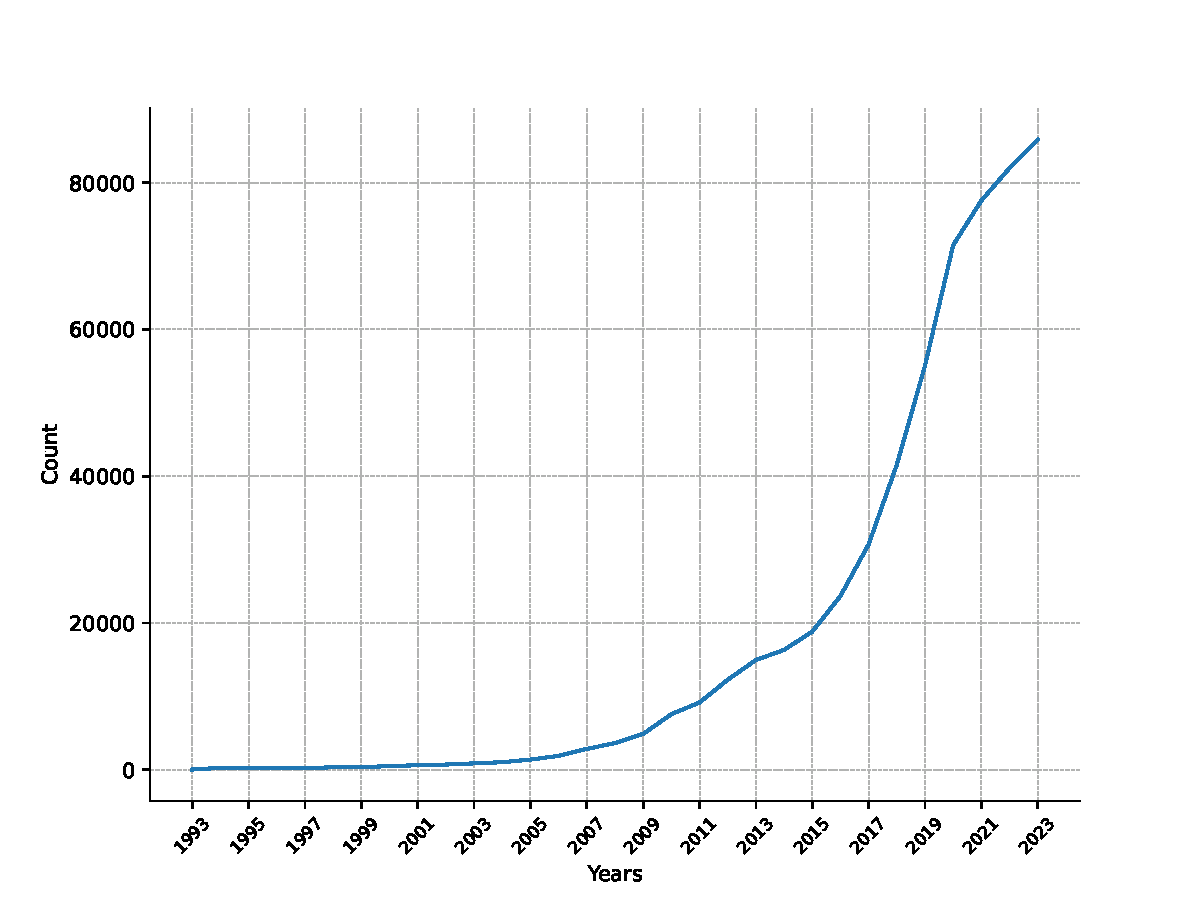
\includegraphics[width=0.99\linewidth]{img/number_of_articles_in_years.pdf}
        \caption{Dynamics of papers in a single category "Computer Science".}
        \label{fig:cumulative}
    \end{figure}
    
    However, such a velocity of publications also requires robust and quick means of search. Currently, there are several ways to find papers and pre-prints related to your field. We will demonstrate the existing search issues with an example: the search of papers related to the quite famous paper \cite{hu2021lora} that introduces the LoRA algorithm for parameter-efficient fine-tuning (PEFT) of large language models (LLM). As we want to find papers that are close to this paper, we perform a search by its title: \textit{Low-rank adaptation of large language models}. For assessment, we evaluate the top 10 answers, ignoring the order. The search was performed on 12/18/2023.
    
    First, is the built-in search on the arXiv platform (Figure \ref{fig:arxiv-search}). Based on the results obtained with a sorting based on decreasing relevance, we can see that only 2 academic papers somehow relate to the paper's content. Other papers are found mostly by matching the words "large language model". Interestingly, we do not see the original paper on the list. So, efficiency is 2/10.

    \begin{figure}[H]
        \centering
        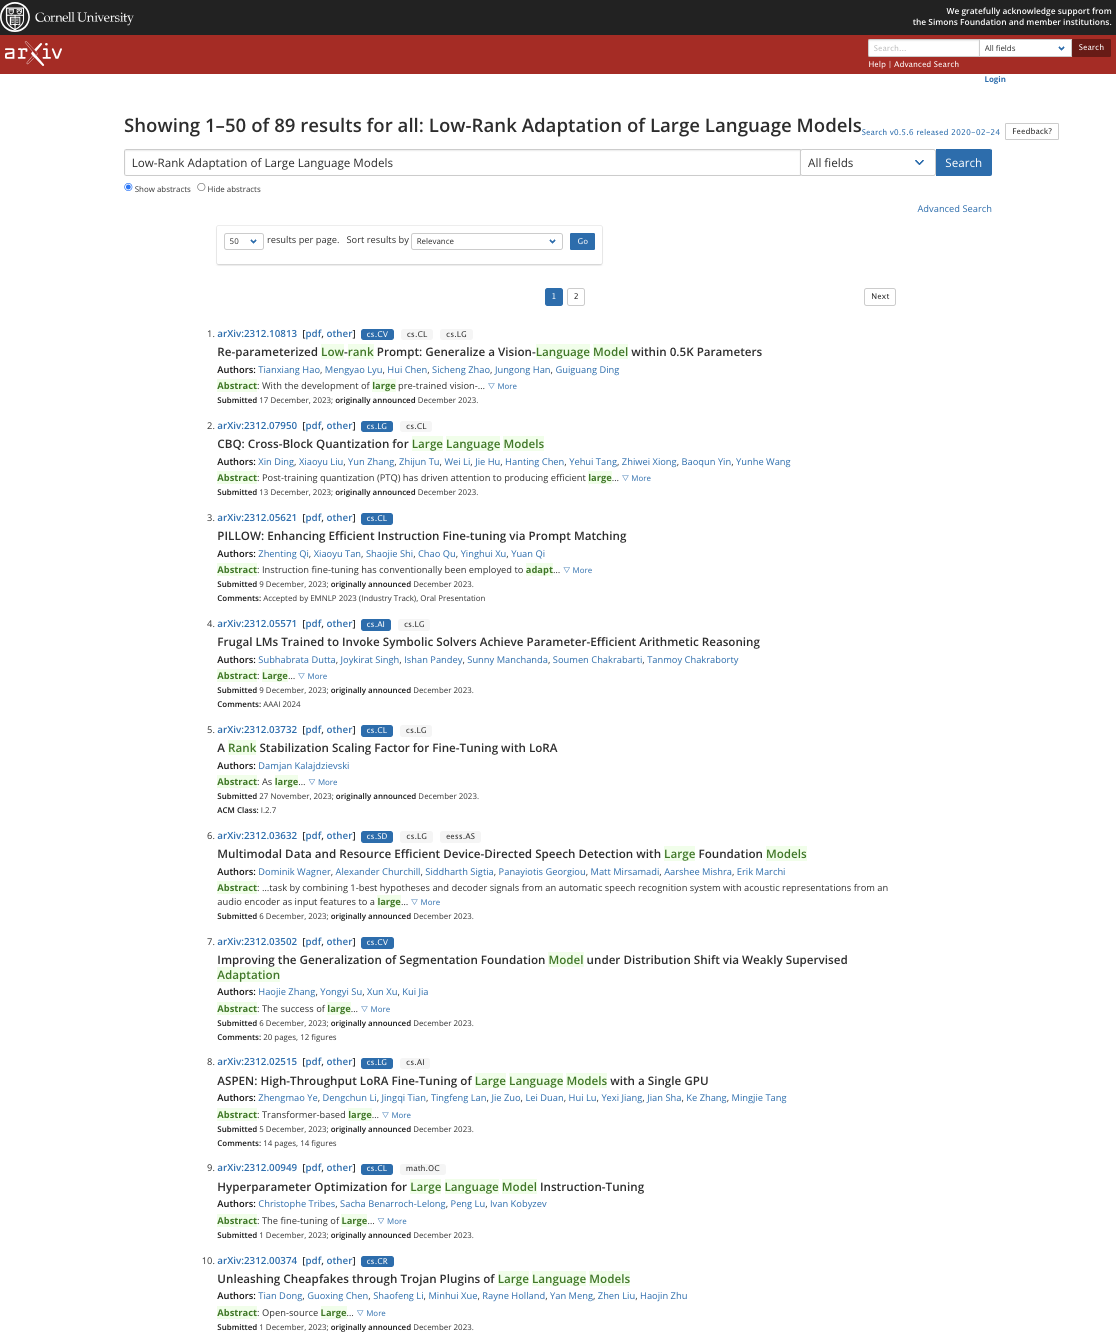
\includegraphics[width=0.89\linewidth]{img/search_arxiv.png}
        \caption{Search by title in arXiv platform.}
        \label{fig:arxiv-search}
    \end{figure}

    The second option is basic search through Google (Figure \ref{fig:google-search}). Based on the results obtained, we can see that only 1 academic paper was found at all, but it is relevant to what we are looking for. Also, we do not count that there are several preprints of the original paper, as we want to find papers that are relevant to that one but not the original paper itself. So, efficiency is 1/10. 
    
    \begin{figure}[H]
        \centering
        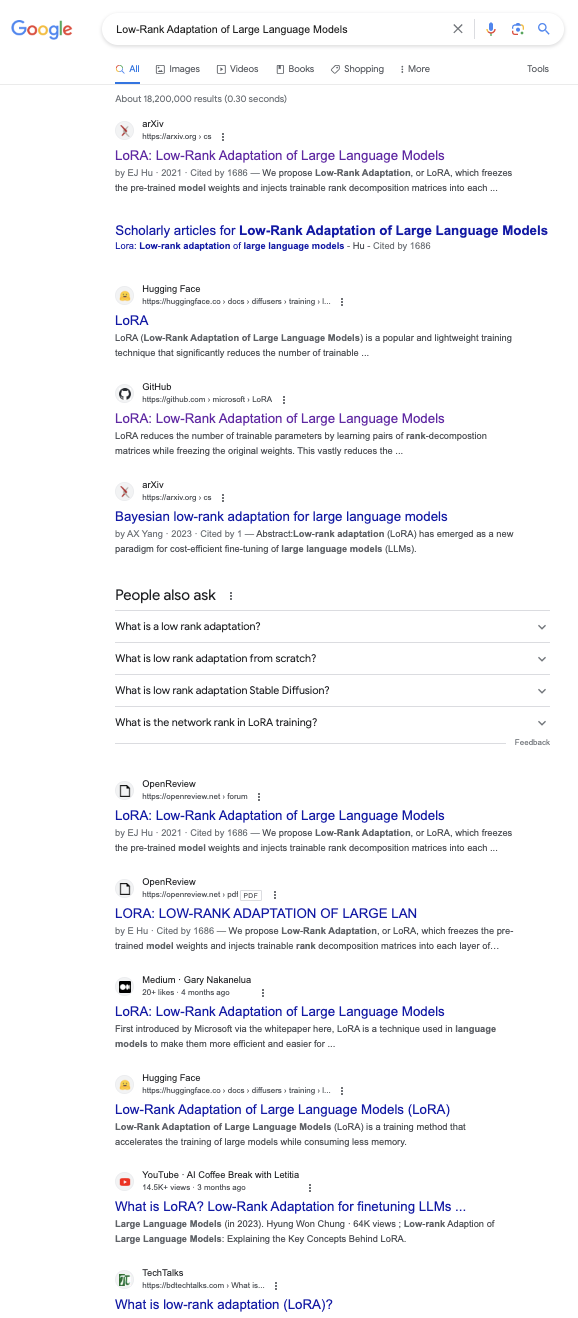
\includegraphics[width=0.6\linewidth]{img/search_google.png}
        \caption{Search by title in Google.}
        \label{fig:google-search}
    \end{figure}

    The third option is advanced search through Google (Figure \ref{fig:advanced-google-search}). As we want to find preprints on a particular website, we can use a special flag in the search query to specify it as the only source for searching, so the query is: \textit{Low-rank adaptation of large language models site:arxiv.org}. Based on the results obtained, we can see that the feed now contains only preprints. After analyzing their relevance to the topic, 6 papers are relevant, 3 are original paper and its duplicates, and 1 is a duplicate of the relevant paper. So, efficiency is 6/10.

    As we can see, the current search engine in arXiv does not help much in finding relevant articles, Google Search allows finding relevant papers much better, but that requires advanced search flags that are not so widespread among researchers, and still, relevance search quality could be further improved. It is hard to predict how exactly Google searches the scientific papers, arXiv seems to search based on keywords.
    
    In this work, we propose a mechanism that allows us to easier and more qualitatively find relevant papers on arXiv. We deliver a prototype of a service for search and plan to suggest integrating it into the built-in search of the arXiv website. We propose to build an index of arXiv papers, use projections of their titles and abstracts to the latent space, and search for relevant papers based on the distance between the distributed representation of a query and the indexed papers.
    
    % 1. why the problem you were working on is important. 
    % 2. what is unique in your approach to this problem,
    % 3. what are the differences to other approaches.

    \subsection{Team}
        \textbf{Alexander Demidovskij} defined the research task and methodology, collected the arXiv index for the Computer Science section from 1993 to 2023, collected a validation dataset based on Google queries, proposed metrics used for model assessment, and prepared this document.

        \textbf{Igor Salnikov} defined a list of deep learning models for comparison, implemented an application, deployed it as an online service, and performed computational experiments with proper visualizations that became an integral part of this document.

    \begin{figure}[H]
        \centering
        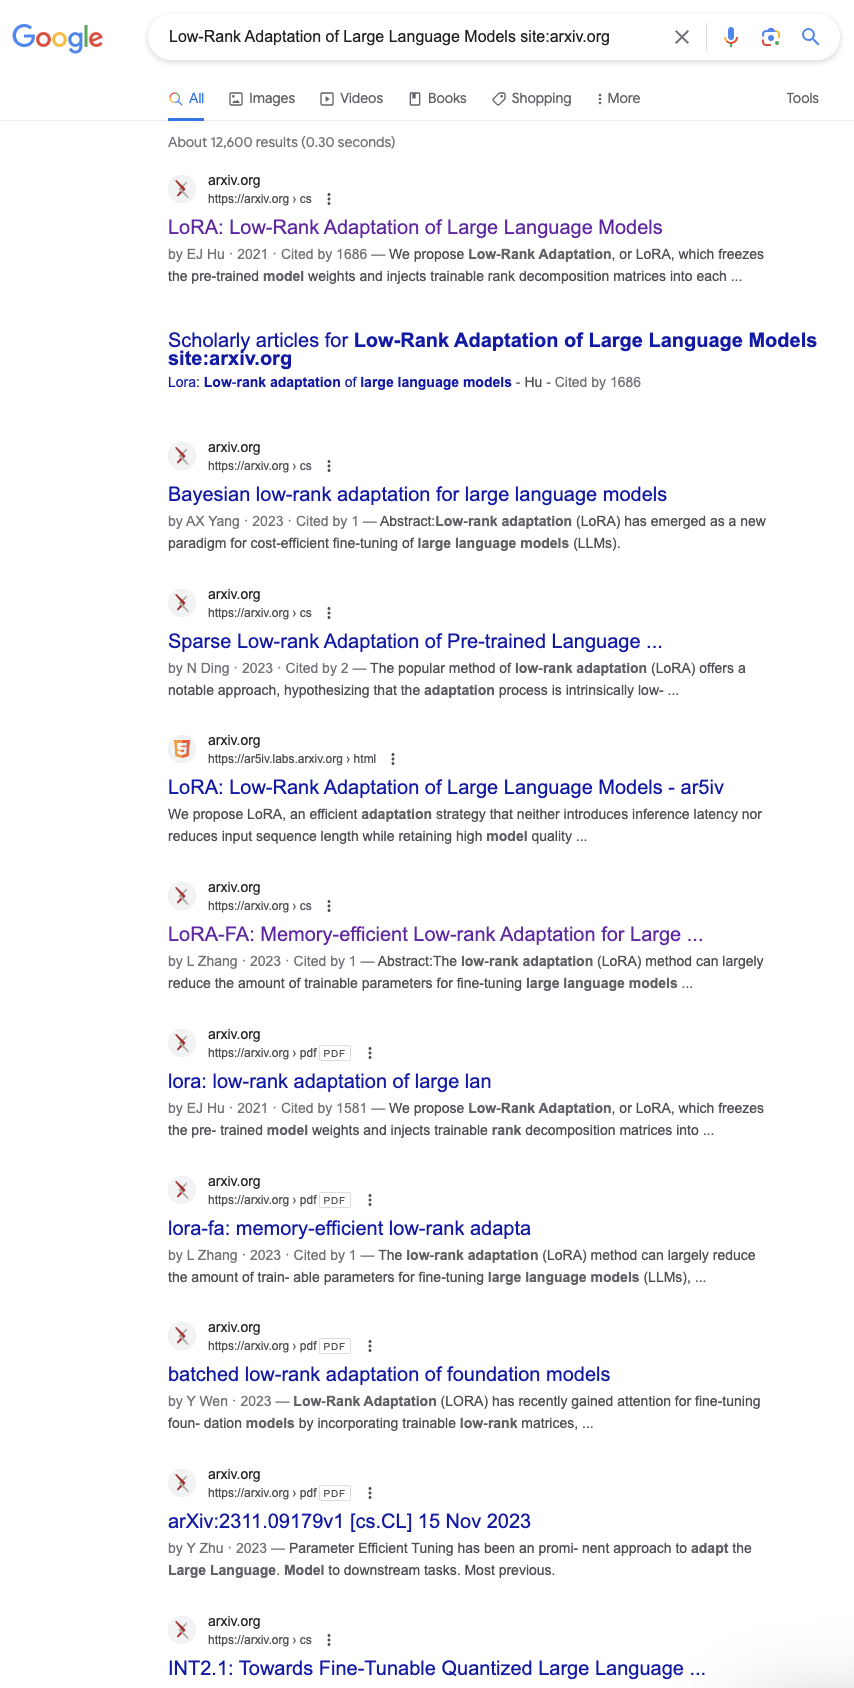
\includegraphics[width=0.65\linewidth]{img/search_google_advanced.png}
        \caption{Search by title in Google with advanced flags.}
        \label{fig:advanced-google-search}
    \end{figure}

\section{Related Work}\label{sec:related}

    Information retrieval (IR) is "the name of the field encompassing the retrieval of all manner of media based on user information needs" \cite{jurafsky}. The task of IR is usually defined by a user's query that is given to the IR system, and the response is a ranked list of documents. 

    Information retrieval has undergone a considerable evolution, starting with term-based methods and ending with the integration of artificial neural networks (ANNs) \cite{zhu2023large}. One of the most basic approaches is keyword retrieval \cite{salton1988term}. Also, within a field of search systems, an important role is played by two ranking approaches: the TF-IDF and BM25 algorithms that define ranking rules for documents based on query terms \cite{robertson1995okapi}. A serious paradigm shift in information retrieval happened due to the introduction of the vector space model \cite{salton1975vector}. The most simple scenario is mapping documents to vectors based on unigram frequencies, and searching is then performed based on the cosine distance between pairs of vectors. The key problem with this approach is the vocabulary mismatch problem: the query contains words that are not known to the system, therefore their statistics become unusable in this case. 
    
    Modern systems are mostly based on ANNs \cite{lin2022pretrained}, but the general principle of using embeddings (or vectorized representations of the text) is the prevailing idea in modern IR systems as well. However, nowadays dense vector representations are obtained with encoder neural networks, such as BERT. However, using pre-trained models, like BERT, might not produce embeddings that capture the semantics of a particular use case. 
    
    One of the key directions is fine-tuning encoders for a downstream task or field. Another important topic in IR is fast indexing and searching of close documents among millions of entries. For example, new libraries appear, such as Facebook's FAISS \cite{faiss} or Nvidia's RAFT \cite{raft}. Designing a production-ready solution in the form of a service or an application is also a challenging task that introduces novel questions to the list of standard design decisions to be made. For example, the selection of algorithms and libraries for efficient search of documents, the selection of a pre-trained encoder, the definition of a distance metric between document embeddings, etc. 

\section{Model Description}\label{sec:methodology}
    We suggest designing the arXiv search engine based on dense embeddings produced by ANN. The proposed system is described according to the key elements of an IR system: rewriter, retriever, reranker, and reader.
    
    \subsection{Rewriter}
    
        We propose to keep the user query as-is, given the assumption that a user is a researcher who needs to find papers exactly about the topic they requested. We recommend introducing an upper bound for a word limit in the query in the same manner as Google does (not more than 32 words). However, no refining of the initial query is needed.

    \subsection{Retriever}
    
        A search for relevant papers should be performed on top of dense representations of papers. The way they are collected and stored is covered in Section \ref{sec:dataset}. Given that all papers have been collected, they should be translated to the latent space with the aid of ANN. We propose to use two strategies. The first one encodes only the title, which is a short and concise summary of the paper. The second one is encoding an abstract - it contains valuable details about the main paper ideas and results; therefore, searching through abstracts might help researchers find related papers based on the query. The number of dimensions of the distributed vector is defined by the encoder architecture.

    \subsection{Reranker}

        We propose to use two different metrics for estimating similarity between query and document: cosine similarity and Euclidean distance (the smaller the distance, the more similar the documents).
        
    \subsection{Reader}

        For academic paper searches, we do not suggest any improvements or rephrasing for the answers exposed to the user. The results of IR are a list of relevant papers that might be interesting for a user.

    
    \subsection{Encoder models}
        
        As for models, we propose to use selected models from HuggingFace. A summary of used models is demonstrated in Table \ref{tab:hf-models}.

        \begin{table}
            \small
            \centering
            \caption[Models selected for the retriever component of arXiv IR]{Models selected for the retriever component of arXiv IR\textsuperscript{*}}
            \small\textsuperscript{*} \url{https://www.sbert.net/docs/pretrained_models.html}
            \label{tab:hf-models}
            \bigskip
            \begin{tabularx}{\textwidth}{XYYYY}
                \toprule
        
                \bfseries Models & \bfseries Max sequence length, tokens & \bfseries Dimensions & \bfseries Speed, sentence/sec & \bfseries Size, MB \\
        
                \midrule
                
                all-MiniLM-L6-v2 &  256 &   384 &   14200 & 80 \\
                all-mpnet-base-v2 & 384 &   768 &   2800 &  420 \\
                all-distilroberta-v1 &  512 &   768 &   4000 &  290 \\
                multi-qa-distilbert-cos-v1 &    512 &   768 &   4000 &  250 \\
                e5-large &  512 &   1024 & N/A &  1340  \\
                \bottomrule
            \end{tabularx}
        \end{table}
    
    \subsection{Quality assessment}
        
        The task of creating a search engine for a particular platform is not a novel one; however, several specific characteristics of the given task for the arXiv platform are still present. First, we do not care at this moment in search engine development about the rank of responses. What is necessary from our point of view is to demonstrate the use of top-N relevant papers for the given query. A similar approach is used in some paid services, such as Connected Papers\footnote{\url{https://www.connectedpapers.com/}} where relevant papers are represented as nodes with an edge between the current paper and the original one. Therefore, ranking metrics are not applicable for evaluating the quality of the final solution.

        Evaluation is not possible without a dataset. For the given task, a new dataset needs to be collected. Technical details on the collection of the validation dataset are given in Section \ref{sec:dataset}. Here, we focus on what should constitute the validation dataset.

        As a query, we considered the title of the article. Complexity comes with the reference answer. We do not want to perform manual annotation, as it does not scale and is error-prone. At the same time, to the best of our knowledge, there is no ready collection of correct recommendations for a given article. We decided to use Google responses as the correct answers. So, for a given article, we get its title, query Google with the special flag as demonstrated in the Introduction, and get top-10 \textit{arXiv} papers from the response. Thus, we obtain a validation dataset entry: a sample (the title of the article) and a reference value (10 arXiv papers). 

\section{Dataset}\label{sec:dataset}
    
    In designing the IR for arXiv papers, we consider the vast amount of papers that should be indexed on a regular basis. So, there is no appropriate source of data other than the content of the arXiv platform available for open access. Therefore, we have designed the scrapper that collects articles from arXiv and collected all articles from January 1993 to November 2023 in the category of "Computer Science".

    The aforementioned scrapper is built on top of a simple scheme of making HTTP GET requests to the pages of the arXiv platform, parsing these pages, and extracting valuable information, such as authors, titles, summary, etc. Now we will explain this process step by step.

    \subsection{Index collection}

        To be able to scrape web data, we need to define the page that contains the necessary information. We are first interested in obtaining a list of papers that were made in a particular month of the particular year. For that, we have identified a proper mechanism on the arXiv platform. When you open the browser with a link \url{https://arxiv.org/list/cs/2301?skip=2000&show=4000}, you will get a list of papers that were published in January (\textbf{01}) 20\textbf{23}, we select to see papers from \textbf{2000}\textsuperscript{th} to \textbf{4000}\textsuperscript{th}. The maximum number of pages is limited by platform and is equal to 2000. Therefore, if we see from the page that in this period there were more than 2000 papers, we make several GET requests to obtain the full list. From the resulting HTML pages, we extract links to the papers and their meta-information. 
        
        The index collection is organized with the help of \textit{requests} and \textit{beautifulsoup4} libraries. All months are processed concurrently with \textit{multiprocessing} module, overall collection time depends on the available cores of the machine. The resulting index is stored in \textit{.csv} format, a separate file for each month and year. At the final stage, these files are joined together with the help of \textit{pandas} library.

        Index collection is performed in a fully automatic manner for a particular category. As a result of the collection, information about 566847 papers was obtained; three of them were filtered out during pre-processing as they are no longer available on the arXiv platform. It is available online\footnote{\url{https://github.com/demid5111/arxiv-ai-search/blob/main/arxiv_scrapper/assets/arxiv_index_Nov_2023.csv}} under GPL-3.0 license. Overall distribution of articles per year in a single category, "Computer Science" is demonstrated in Figure \ref{fig:articles-pie}.

        \begin{figure}[H]
            \centering
            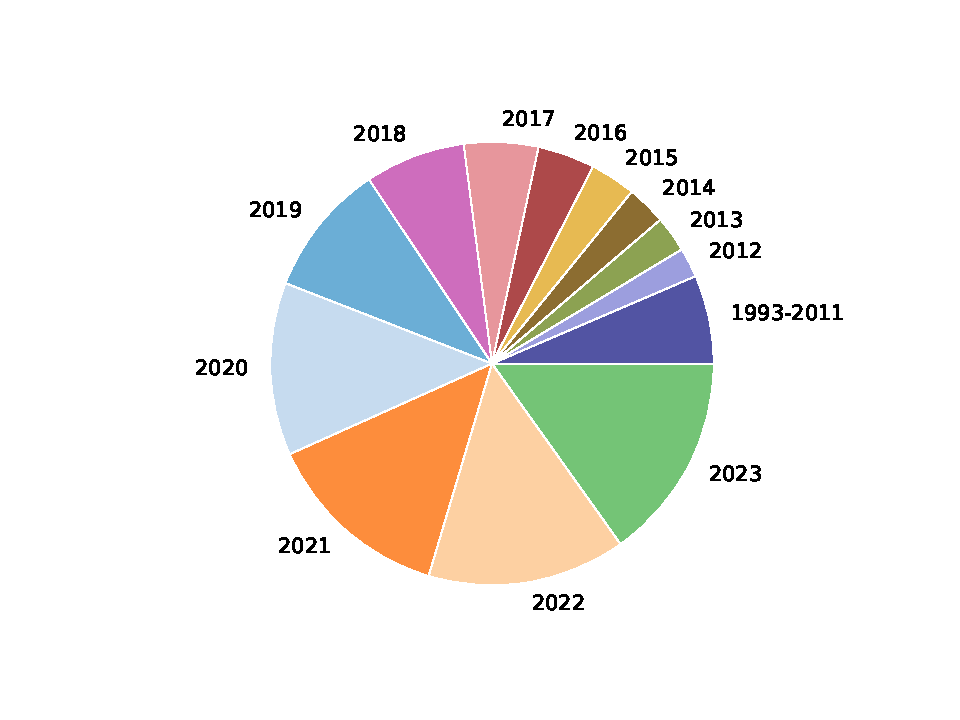
\includegraphics[width=0.99\linewidth]{img/articles_in_every_year.pdf}
            \caption{Overall distribution of articles per year in a single category "Computer Science".}
            \label{fig:articles-pie}
        \end{figure}

    \subsection{Abstracts collection}

        Original HTML pages with a list of papers published in a particular month do not contain abstracts. Therefore, we need to collect abstracts for each paper separately. The overall approach is the same: a GET request to obtain an HTML page with an abstract, parsing the HTML, and extracting vital information. To give an example of a page that contains an abstract, we refer to \url{https://arxiv.org/abs/2106.09685}.

        Abstract collection is organized with the help of \textit{requests} and \textit{beautifulsoup4} libraries. All months are processed concurrently with \textit{multiprocessing} module, overall collection time depends on the available cores of the machine. However, it is considerably long: it takes 3--4 machine days on moderate hardware (8--16 CPU cores). The resulting file is stored in \textit{.csv} format, a separate file for each month and year. At the final stage, these files are joined together with the help of \textit{pandas} library.

        Abstract collection is performed in a fully automatic manner for a particular category. As a result of the collection, abstracts of 566847 papers were obtained; three of them were filtered out during pre-processing as they are no longer available on the arXiv platform. The dataset is available online\footnote{\url{https://cloud.mail.ru/public/MrJu/TW2mYSV55/arxiv_abs_Nov_2023.csv}} under GPL-3.0 license. The overall distribution of articles per month through whole period of arXiv existence in a single category "Computer Science" is demonstrated in Figure \ref{fig:articles-bars}.

        \begin{figure}[H]
            \centering
            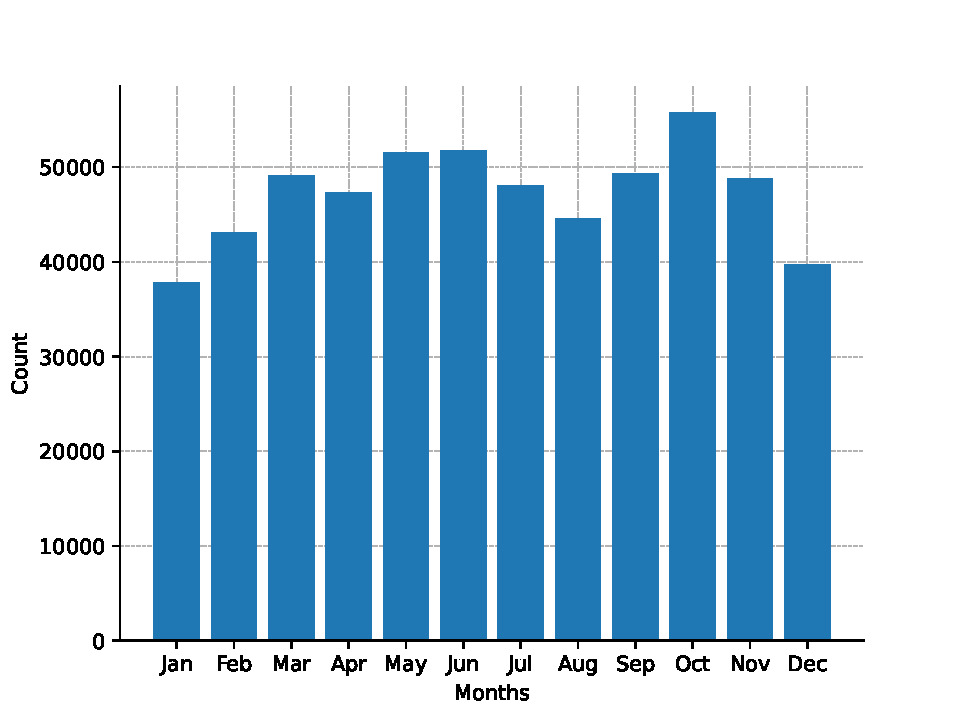
\includegraphics[width=0.8\linewidth]{img/number_of_articles_by_month.pdf}
            \caption{Overall distribution of articles per month in a single category "Computer Science".}
            \label{fig:articles-bars}
        \end{figure}

    
    \subsection{Validation dataset collection}

        As described in Section \ref{sec:methodology}, we are measuring the performance of our system with the help of a special procedure for alignment with Google search results. During the design of the validation dataset, we faced several issues:
        
        \begin{enumerate}
            \item Google is very strict with GET requests made from code. After 3--10 successful requests, Google bans the IP for approximately 8--12 hours.
            \item Google's HTML names (styles, classes) are auto-generated and change almost in every response. 
        \end{enumerate}

        To tackle these problems, we have chosen a different scraping strategy. Instead of a GET request from Python code, we open a browser in headless mode via \textit{selenium} library, open a page in the browser, get HTML from the browser, and only then parse it. Working from a browser allows you to make much more requests (up to 30) per IP. Also, we open a browser with a special URL that already contains a search string, so we skip the additional step of searching, which saves an additional 20--30 requests and allows us to make up to 60 requests per single IP. So, to collect a validation dataset for 12 months with 10 entries per month, we need two IP addresses. Obviously, it does not perfectly scale and requires running this scrapper on several machines. At the same time, it is still much faster and safer than collecting the same amount of validation data with the help of human annotators, such as students.

        The validation dataset contains entries from 2019--2023, takes nearly 12 hours, and needs 10 unique IP addresses. As a result of collection, the validation dataset contains 590 entries, after pre-processing, 235 are left. It is available online\footnote{\url{https://github.com/demid5111/arxiv-ai-search/blob/main/arxiv_scrapper/assets/arxiv_google_Nov_2023.csv}} under GPL-3.0 license.

\section{Experiments}

    \subsection{Metrics}
    
        We have defined the following metrics for evaluating the quality of our solution.

        \paragraph{Precision}
       
            For true positives (\(TP\)) we consider papers that are both in the reference list and in predictions, (\(FP\)) we consider papers that are not in the reference list but are present in predictions. We evaluate precision according to (\ref{eq:precision}).


            \begin{equation}
                Precision = \frac{|TP|}{|TP| + |FP|}
                \label{eq:precision}
            \end{equation}

        \paragraph{Hits@K}
       
            We evaluate Hits@K according to (\ref{eq:top-k}), where \(D\) denotes dataset, \(x, Y\) -- a query and reference results from a single entry of validation dataset, \(\phi\) -- search function.

            \begin{equation}
                \begin{split}
                    hit(Y, \hat{Y}, k) &= \left\{\begin{matrix}
                        1, & | Y \cap \{\hat{y_{i}} \in \hat{Y} | i=1,2,...,k\} | > 0 \\
                        0, & otherwise \\
                       \end{matrix}\right. \\ 
                    Hits(D, k) &= \frac{\sum_{x, Y \in D} hit(Y, \phi(x), k)}{|D|}
                \end{split}
                \label{eq:top-k}
            \end{equation}

    \subsection{Experiment Setup}
        
        Hardware used for experiments: CPU: AMD Ryzen 3 PRO 3200G X4 3.6GHz, GPU: NVIDIA GeForce RTX 3060 12 GB. Software used for experiments: driver version: 525.147.05, CUDA version: 12.0.  Models were taken from HuggingFace (Table \ref{tab:hf-models}). Dataset details are present in Section \ref{sec:dataset}. The encoding of papers was performed on a GPU. The number of \(K\) in metrics is defined as 1 and 10.
    
    \subsection{Baselines}
            
        As a baseline, we consider a random selection of related papers. The number of related papers is defined as 10. 
    
    \section{Results}
        We have performed extensive experiments with the own scrapped validation dataset, and we have built a prototype of a service that is available online for free use. The validation dataset is stored in a vectorized database, and search is performed based on similarity between the vector representation of the query and the paper. The query content varies; it can be either an abstract or the title of a paper for which we want to find similar works. Every paper in the database is always represented as a vector representation of its abstract. We have performed 4 experiments with each encoder model, resulting in 20 experiments. Each experiment is searched for similar papers by the original one. All experiments are grouped by configuration.
        
        \begin{enumerate}
            \item Search by original paper abstract, \(L_{2}\) as a distance metric (Table \ref{tab:experiments:abs-l2}),
            \item Search by original paper abstract, \(cosine\) as a distance metric (Table \ref{tab:experiments:abs-cos}),
            \item Search by original paper title, \(L_{2}\) as a distance metric (Table \ref{tab:experiments:title-l2}),
            \item Search by original paper title, \(cosine\) as a distance metric  (Table \ref{tab:experiments:title-cos}).
        \end{enumerate}
    
        \begin{table*}[!htbp]
    \small
    \centering
    \caption{Experiment results for search by indexed abstracts with \(L_{2}\) as a distance.}

    \begin{tabularx}{0.99\textwidth}{XIII}

        \toprule

        \bfseries Model & \bfseries Precision, \% & \bfseries Hit@K, \% & \bfseries Accuracy, \% \\

        \midrule
        
        all-MiniLM-L6-v2	& 21.15 &	99.15 &	99.15 \\
        all-mpnet-base-v2	& 21.53 &	99.57 &	99.57 \\
        all-distilroberta-v1	& 21.79 &	99.15 &	99.15 \\
        multi-qa-distilbert-cos-v1	& 19.15 &	97.87 &	97.02 \\
        e5-large	& 22.47 &	98.3  &	98.3 \\

        \bottomrule

    \end{tabularx}

    \label{tab:experiments:abs-l2}
\end{table*}

\begin{table*}[!htbp]
    \small
    \centering
    \caption{Experiment results for search by indexed abstracts with \(cosine\) as a distance.}

    \begin{tabularx}{0.99\textwidth}{XIII}

        \toprule

        \bfseries Model & \bfseries Precision, \% & \bfseries Hit@K, \% & \bfseries Accuracy, \% \\

        \midrule
        
        all-MiniLM-L6-v2	& 21.15 &	99.15 &	99.15 \\
        all-mpnet-base-v2	& 21.53 &	99.57 &	99.57 \\
        all-distilroberta-v1	& 21.79 &	99.15 &	99.15 \\
        multi-qa-distilbert-cos-v1	& 19.15 &	97.87 &	97.02 \\
        e5-large	& 22.47 &	98.3  &	98.3 \\

        \bottomrule

    \end{tabularx}

    \label{tab:experiments:abs-cos}
\end{table*}

\begin{table*}[!htbp]
    \small
    \centering
    \caption{Experiment results for search by indexed titles with \(L_{2}\) as a distance.}

    \begin{tabularx}{0.99\textwidth}{XIII}

        \toprule

        \bfseries Model & \bfseries Precision, \% & \bfseries Hit@K, \% & \bfseries Accuracy, \% \\

        \midrule
        
        all-MiniLM-L6-v2	& 21.15 &	99.15 &	99.15 \\
        all-mpnet-base-v2	& 21.53 &	99.57 &	99.57 \\
        all-distilroberta-v1	& 21.79 &	99.15 &	99.15 \\
        multi-qa-distilbert-cos-v1	& 19.15 &	97.87 &	97.02 \\
        e5-large	& 22.47 &	98.3  &	98.3 \\

        \bottomrule

    \end{tabularx}

    \label{tab:experiments:title-l2}
\end{table*}

\begin{table*}[!htbp]
    \small
    \centering
    \caption{Experiment results for search by indexed titles with \(cosine\) as a distance.}

    \begin{tabularx}{0.99\textwidth}{XIII}

        \toprule

        \bfseries Model & \bfseries Precision, \% & \bfseries Hit@K, \% & \bfseries Accuracy, \% \\

        \midrule
        
        all-MiniLM-L6-v2	& 21.15 &	99.15 &	99.15 \\
        all-mpnet-base-v2	& 21.53 &	99.57 &	99.57 \\
        all-distilroberta-v1	& 21.79 &	99.15 &	99.15 \\
        multi-qa-distilbert-cos-v1	& 19.15 &	97.87 &	97.02 \\
        e5-large	& 22.47 &	98.3  &	98.3 \\

        \bottomrule

    \end{tabularx}

    \label{tab:experiments:title-cos}
\end{table*}

    
        Based on the results of the experiments, for the task of searching similar papers by title, the best performing model is \textit{e5-large} as it allows achieving 85.96\% Hits@10 for search by title, 58.72\% Hits@1 and 21.45\% precision. For the task of searching similar papers by abstract, the best performing model is \textit{all-mpnet-base-v2} as it allows achieving 99.57\% Hits@10 for search by title, 99.57\% Hits@1.
    
        Moreover, as can be seen from tables, there is practically no difference in the \(L_{2}\) and \(cosine\) metrics and is observed only for some models in ten-thousandth orders.
    
        It is also important to compare the performance of the resulting solution on the same example as we used in the Introduction to demonstrate the beneficial behavior of the new system (Figure \ref{fig:aziri-search}). Based on the results obtained, eight papers are relevant, and two are less relevant but still interesting for an expert in the PEFT field. So, efficiency is 8/10.
    
        The service is a client-server application. The client part is a search form and fields for displaying results. Written using JavaScript and the Bootstrap5 library as a CSS framework. The server part uses the FastAPI framework as a backend, and ChromaDB as a vector database. A model: e5-large was used to generate embeddings and fill the database with data. Prototype of the service is deployed and available online: \url{http://62.84.112.56:8000/}.
        
    
    \section{Conclusion}
    
        In this work, we have proposed a novel approach to finding relevant preprints on the arXiv platform. In particular, we have the following contributions:
        
        \begin{enumerate}
            \item identified a problem in the search for relevant papers by manually comparing their quality on arXiv and Google,
            \item proposed a solution based on dense vector representations obtained by modern encoder-based neural networks,
            \item designed an automatic scrapper of arXiv papers that scales to the whole platform and to the available hardware,
            \item collected a full index of arXiv papers for a period of its existence (1993-nowadays) in a section "Computer Science" (566844 papers),

            \begin{figure}[H]
                \centering
                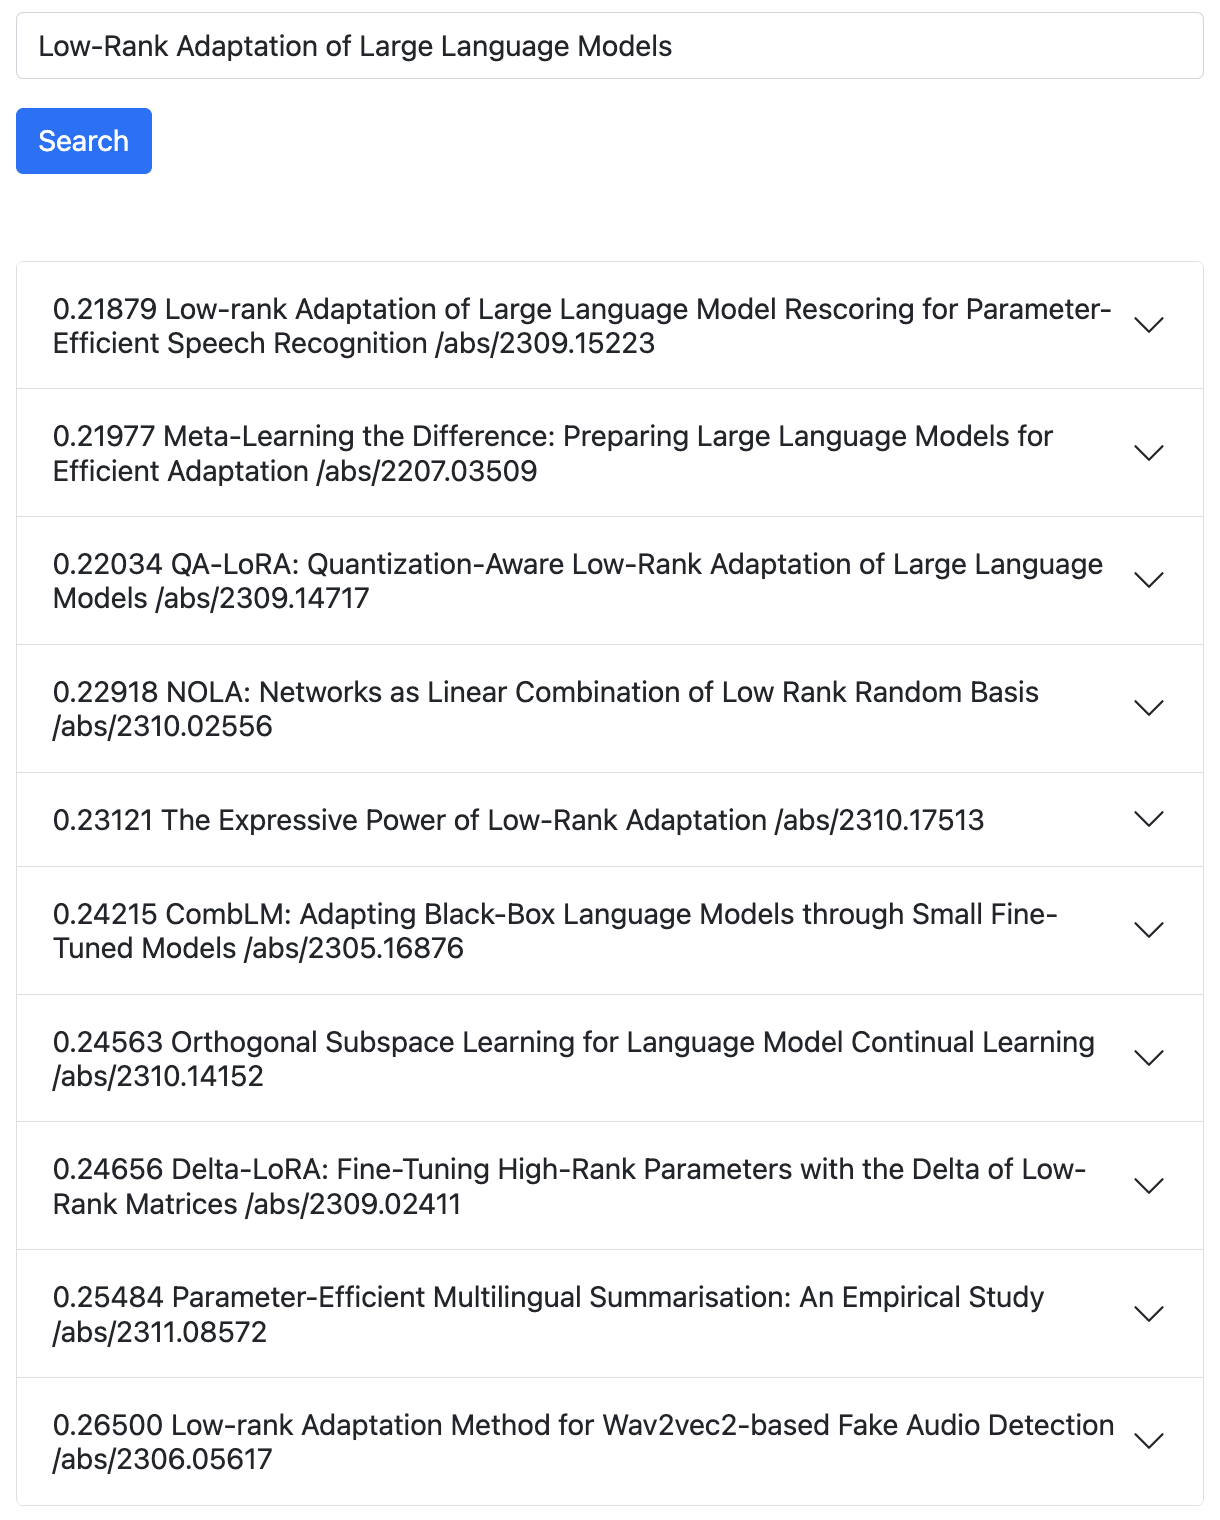
\includegraphics[width=0.8\linewidth]{img/search_aziri.png}
                \caption{Search by title in proposed service.}
                \label{fig:aziri-search}
            \end{figure}

            \item identified an original approach to evaluating the quality of search via Google search feed,
            \item collected a validation dataset based on the specially designed approach of hybrid (both static and dynamic scrapping),
            \item performed computational experiments with the validation dataset and 5 deep learning pre-trained models and identified the best-performing model, which is \textit{e5-large},
            \item designed a system for efficient storage and search of documents based on their distributed representation,
            \item designed and deployed a prototype of the web service that demonstrates the capabilities of the search and is free to use. A prototype of the service is deployed and available online: \url{http://62.84.112.56:8000/}.
        \end{enumerate}

        
        
        We want to believe that our work might be integrated into the arXiv or continue to exist as a standalone service. There are multiple directions for further research: indexing whole paper content instead of just abstracts; improving metrics and introducing rank-based metrics for quality assessment; regular scans of the arXiv platform, service robustness and stability; etc. We are sure that our contribution to the arXiv as a leading preprint platform will help researchers find relevant papers easier, which will allow better and faster information exchange and bring more innovation. 
    
\bibliographystyle{apalike}
\bibliography{lit}
\end{document}
